\textcolor{red}{Erich: Is this important?  Should we take it out? So what if the matrix is banded?  What advantages does this bring?}
Different node orderings in a mesh correspond to permutations of the stiffness
matrix. 
Since memory use and convergence speed of iterative methods may
depend on the ordering used, it is important to pick a node number that is most
efficient (see, e.g., Fairag \emph{et. al.} \cite{Fairag}). 
The node numbering used in this report is that used in \cite{Fairag}, since it was shown there that it
results in a banded stiffness matrix.

The node ordering consisted of first numbering the vertices of each triangle
with six successive numbers and then numbering the midpoint nodes starting
with the horizontal sides, followed by the vertical and oblique sides. An
illustration of the node numbering can be found in \autoref{fig:MatrixGraph}.
This node numbering results in a banded matrix that can be seen graphically in
\autoref{fig:MatrixGraph}.

\begin{figure}[h]
	\begin{center}
    \begin{tikzpicture}[scale=0.4]
\tikzstyle{every node}=[font=\tiny]
      \draw (0,0) node[below left,fill=none]
      {$\begin{array}{l}1,\\2,3\\4,5,6\end{array}$} 
      -- (3,0) node[below,fill=none] {$25$}
      -- (6,0) node[below right,fill=none]
      {$\begin{array}{l}7,\\8,9\\10,11,12\end{array}$} 
      -- (6,3) node[above right,fill=none] {$29$}
      -- (6,6) node[above right,fill=none] 
      {$\begin{array}{l}19,\\20,21\\22,23,24\end{array}$} 
      -- (3,6) node[above,fill=none] {$26$}
      -- (0,6) node[above left,fill=none]
      {$\begin{array}{l}13,\\14,15\\16,17,18\end{array}$} 
      -- (0,3) node[above left,fill=none] {$27$}
      -- cycle;
      \draw (0,0) -- (3,3) node[above left,fill=none] {$28$} -- (6,6);
    \end{tikzpicture}	
    \hspace*{0.8cm}
    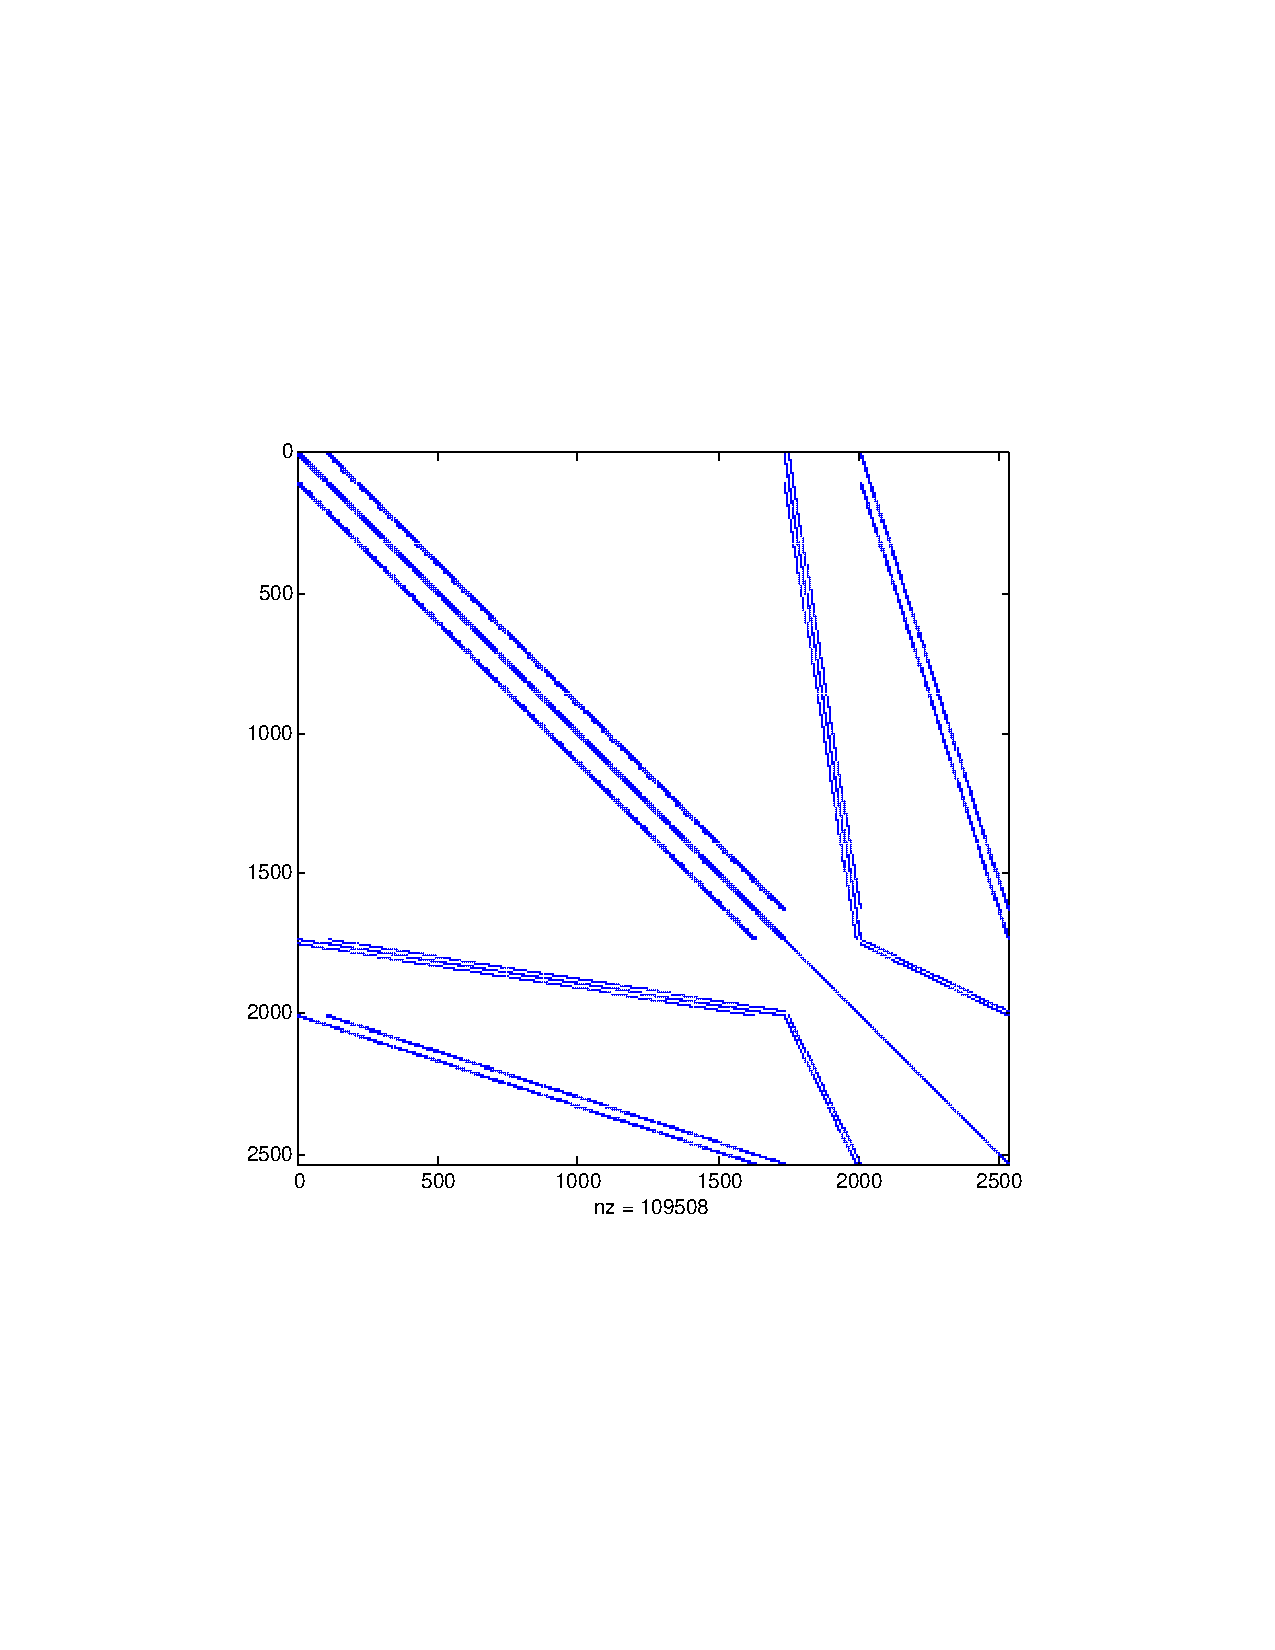
\includegraphics[trim=100 200 100 210, clip, scale=0.35]{Matrix.pdf}
	\end{center}
  \caption{
  Example of element global node numbering (left) and resulting stiffness matrix (right).
  }
	\label{fig:MatrixGraph}
\end{figure}

